\chapter{Fundamental Mathematics and Notation}
\label{chap:fundamentals} 
It is necessary to recall some fundamental mathematical concept to understand the subsequent chapters and introduce the notations used in the thesis.
This chapter introduces the essential mathematical backgrounds that are directly relevant to the contents of this thesis to help readers to a clear understanding of the subsequent chapters.
The theoretical discussion will often appear with minimal definition and citation of the details works since details discussion is beyond the scope of this thesis.
For more details of the topics discussed in this chapter we refer to \cite{lidl_niederreiter_1996, book_HFFMullen2013}.
As an additional purpose, this chapter specifies most of the notations that will appear in the upcoming chapters.

Cryptography deals with numbers mostly integers.
To understand modern cryptography  it is essential to have a good understanding of the  underlying mathematical concepts. 
The following concepts is the basic for the discussion of the subsequent chapters.

\section{Modular Arithmetic}
\label{sec:chap:fund:modular_arithm} 
 Modular arithmetic is the fundamental tool for modern cryptography specially public key cryptosystems.
\begin{definition}[Modular Arithmetic\index{modulus}]
	Let  $p$ be a positive integer named as the modulus \index{modulus} and  $a$ and $b$  are two arbitrary integers. 
	If  $p$ divides $b-a$  then we can write
	 $$ a \equiv b ~(\bmod ~p)$$
	 and express as $a$ and $b$ are congruent modulo $p$.
\end{definition}
\begin{example}
	Let, $p =7$, $a=19$ and $b=5$ then 
	$19  \equiv  5 ~(\bmod ~7) $.
\end{example}

\begin{example}
	Let, $p =7$, $a=-17$  and $b=11$. Then $-17  ~(\bmod ~7)  = 4$ and $11 ~(\bmod ~7) = 4$. 
	We can write 
	$$-17  \equiv  11 ~(\bmod ~7) $$ 
	and usually express $-17$ and $11$ are congruent modulo $7$.
\end{example}

\section{Group, Ring, Field}
\label{sec:chap:fund:group}
\subsection{Group}
The concept of group \index{group} is very fundamental for understanding cryptography. It is an algebraic system defined as follows.
\begin{definition}[Group\index{group}]
A group \index{group} is a non empty set $\mathbb{G}$ with a binary operation $\circ$ on its elements denoted as  $\langle\mathbb{G}\index{group},\circ\rangle$,  sometimes denoted by   $\mathbb{G}$ only, which satisfies the following axioms.
\begin{quote}
	\begin{description}
		\item[Closure] The group is closed under the operation $\circ$, i.e.  $\forall a \in\mathbb{G}$, and $\forall b \in\mathbb{G}$ the result of $ (a\circ b) = c \in \mathbb{G}$. \footnote{$\forall$ symbol bears is usual notation \textit{"for all"} }
		
		\item[Identity element] There exist an \textbf{identity element \index{Identity element}} $e$ also know as \textit{neutral element} or \textit{unit element} in $\mathbb{G}$ such that $\forall a \in\mathbb{G} \index{group}$,  $a\circ e = e\circ a = a$.
		
		\item[Inverse element] For ${\forall}a \in\mathbb{G}\index{group}$, there exists an element $b\in\mathbb{G}\index{group}$ such that $a\circ b=e=b\circ a$, where $b$ is called inverse element of $a$.
		
		\item[Associativity] Elements in  group $\mathbb{G}$ should follow associativity. i.e. $(a\circ b)\circ c=a\circ (b\circ c)$ for all $ a,b,c\in\mathbb{G}\index{group}$.
		
\end{description}
\end{quote}
\end{definition}

\begin{definition}[Commutative Group\index{group}] \hspace{0em}
\begin{quote}\begin{description}
A group \index{group} $\mathbb{G}\index{group}$ will be commutative if $a\circ b=b\circ a$ for all $a,b \in\mathbb{G}\index{group}$.
\end{description}\end{quote}
\qed
\end{definition}
A commutative group is also called \textit{abelian} group.

\begin{example} \label{example_group}
 The set of integers $\mathbb{Z}$ forms a group under the group operation of addition $+$ denoted as $(\mathbb{Z},+)$. $0$ is the identity element of the group.
\end{example}
\begin{example}\label{example_notgroup}
	 The set of positive integers $\mathbb{N}$ under addition does not form a group since elements have not inverse.
\end{example}
%For example, the algebraic system $\langle\mathbb{Z},+\rangle$ is an infinite commutative group\index{group}, where $\mathbb Z$ is the integer set and $+$ means the ordinary addition for integers. For a finite group\index{group}, its order\index{group order} is defined as follows.
\begin{definition}[Order of a Group\index{group}]\hspace{0em}
The order of a group $\mathbb{G}$ \index{group order} often denoted as $\#\mathbb{G}\index{group}$ is the number of elements in the group\index{group} $\mathbb{G}\index{group}$.
\qed
\end{definition}

\begin{remark}
	 Groups order can be finite and infinite. In example \ref{example_group}, $(\mathbb{Z},+)$ has infinite order.
\end{remark}

\begin{definition}[Order of group element\index{order of element}]
	For an element $a\in\mathbb{G}\index{group}$, the smallest positive integer $m$ such that $a^{m}=e$ is called the order\index{order} of $a$, where $e$ is the identity element in $\mathbb{G}\index{group}$.
	\qed
\end{definition}

\begin{example}{Finite group:  \index{finite group} } \label{definition_finite_group}
As shown in example \ref{example_notgroup}, the set $\mathbb{N}$ under addition does not form a group 
since it does not satisfy the group\index{group} axioms. 
Let us consider a set $\mathbb{N}_{n}$ under the operation $\mod n$  such that 
$$ \mathbb{N}_{n} = \{0,1,2,3, \cdots, n-1\}$$
where $n \in \mathbb{N}$.
It means $\mathbb{N}_{n}$ is the set of remainders under ``$\bmod\ n$''.
Recall the modular arithmetic that 
$$a+b\equiv c\ \ \bmod n\hspace{3em}a,b\in \mathbb{N}_{n},\label{Sum Definition}$$
 means $c$ is  associated to a remainder on division by $n$ when $a+b=c\notin\mathbb{N}_{n}$. 
It makes $c$ belongs to $\mathbb{N}_{n}$ making $( \mathbb{N}_{n},+)$ forming a group\index{group}.
In also includes element $0$ which acts as an identity element.
\end{example}

\begin{definition}[Group generator\index{group}]
	For a given group\index{group} $\mathbb{G}\index{group}$ if there is an element $g\in\mathbb{G}\index{group}$ such that for any $a\in\mathbb{G}\index{group}$ there exist an unique integer $i$ with $a=g^{i}$ then $g$ will be called a   generator\index{generator} of  $\mathbb{G}\index{group}$
\qed
\end{definition}

\begin{definition}[Cyclic Group\index{group}]
A group\index{group} $\mathbb{G}\index{group}$ will be {\em cyclic} if there exist at least one generator $g \in \mathbb{G}$. Cyclic group usually expressed as $\mathbb{G} = \langle g \rangle$
 \qed 
\end{definition}

\begin{remark}
	The number of generator in a group $\mathbb{G}\index{group}$ of order $n$ is defined by Euler's totient function $\phi(n)$\footnote{When $n$ is a positive integer, Euler's totient function $\phi(n)=$ number of positive integers less than or equal to $n$ that are co-prime to $n$}.
	If $n$ is a prime $p$ then the  group $\mathbb{G}$ will be called prime order group and it will have $\phi(p) = p-1$ generators.
\end{remark}

\begin{definition}[Cyclic Group\index{group}]
	A group\index{group} $\mathbb{G}\index{group}$ will be {\em cyclic} if there exist at least one generator $g \in \mathbb{G}$. Cyclic group usually expressed as $\mathbb{G} = \langle g \rangle$ 
	\qed 
\end{definition}

In this case we use the notation $\langle\mathbb{G}\index{group},\circ\rangle$,  there exists some ambiguity which operation we consider.
Therefore, the following two types of group nations are very common in literature.

\begin{definition}[Additive group\index{additive group}]
A cyclic group is called \textit{additive} if we tend to write its group operation in the same way we do additions, that is 
$$f = g + x$$ 
can also appear as $[x]g$ meaning applying $x -1$ times addition operator $+$ on $g$.
It is also common to write as $x \cdot g$.
For example, $1$ is one of generators in group $(\mathbb{Z}_5, + )$ under addition modular $5$, then $1 \cdot 4$ can be written as $$ 4 = 1+ 1+ 1+1.$$
\qed
 \end{definition}

\begin{definition}[Multiplicative group\index{multiplicative group}]
	A cyclic group is called \textit{multiplicative} if we tend to write its group operation in the same way we do multiplication, that is 
	$$f =  g \cdot x ~\text{or}~ f = g^x$$ 
	\qed
\end{definition}

\begin{remark}
	In both notation the $x$  is an integer called the \textit{discrete logarithm} of $h$ to the base $g$.
\end{remark}
\begin{remark}
	Unless otherwise stated, through out this thesis we will use the $xg$ notation for ordinary addition e.g. $a+a=2a$ and $a+a+a=3a$ and for multiplicative notation, these will denoted by $a^2$, $a^3$.
\end{remark}

From the definition cyclic group, it can be see visualized that any elements in cyclic a group\index{cyclic group} are generated with iterative operations of generator\index{generator} $g$. 
\fgref{Cyclic group} shows this schematically.
\begin{figure}[ht]
\begin{center}
	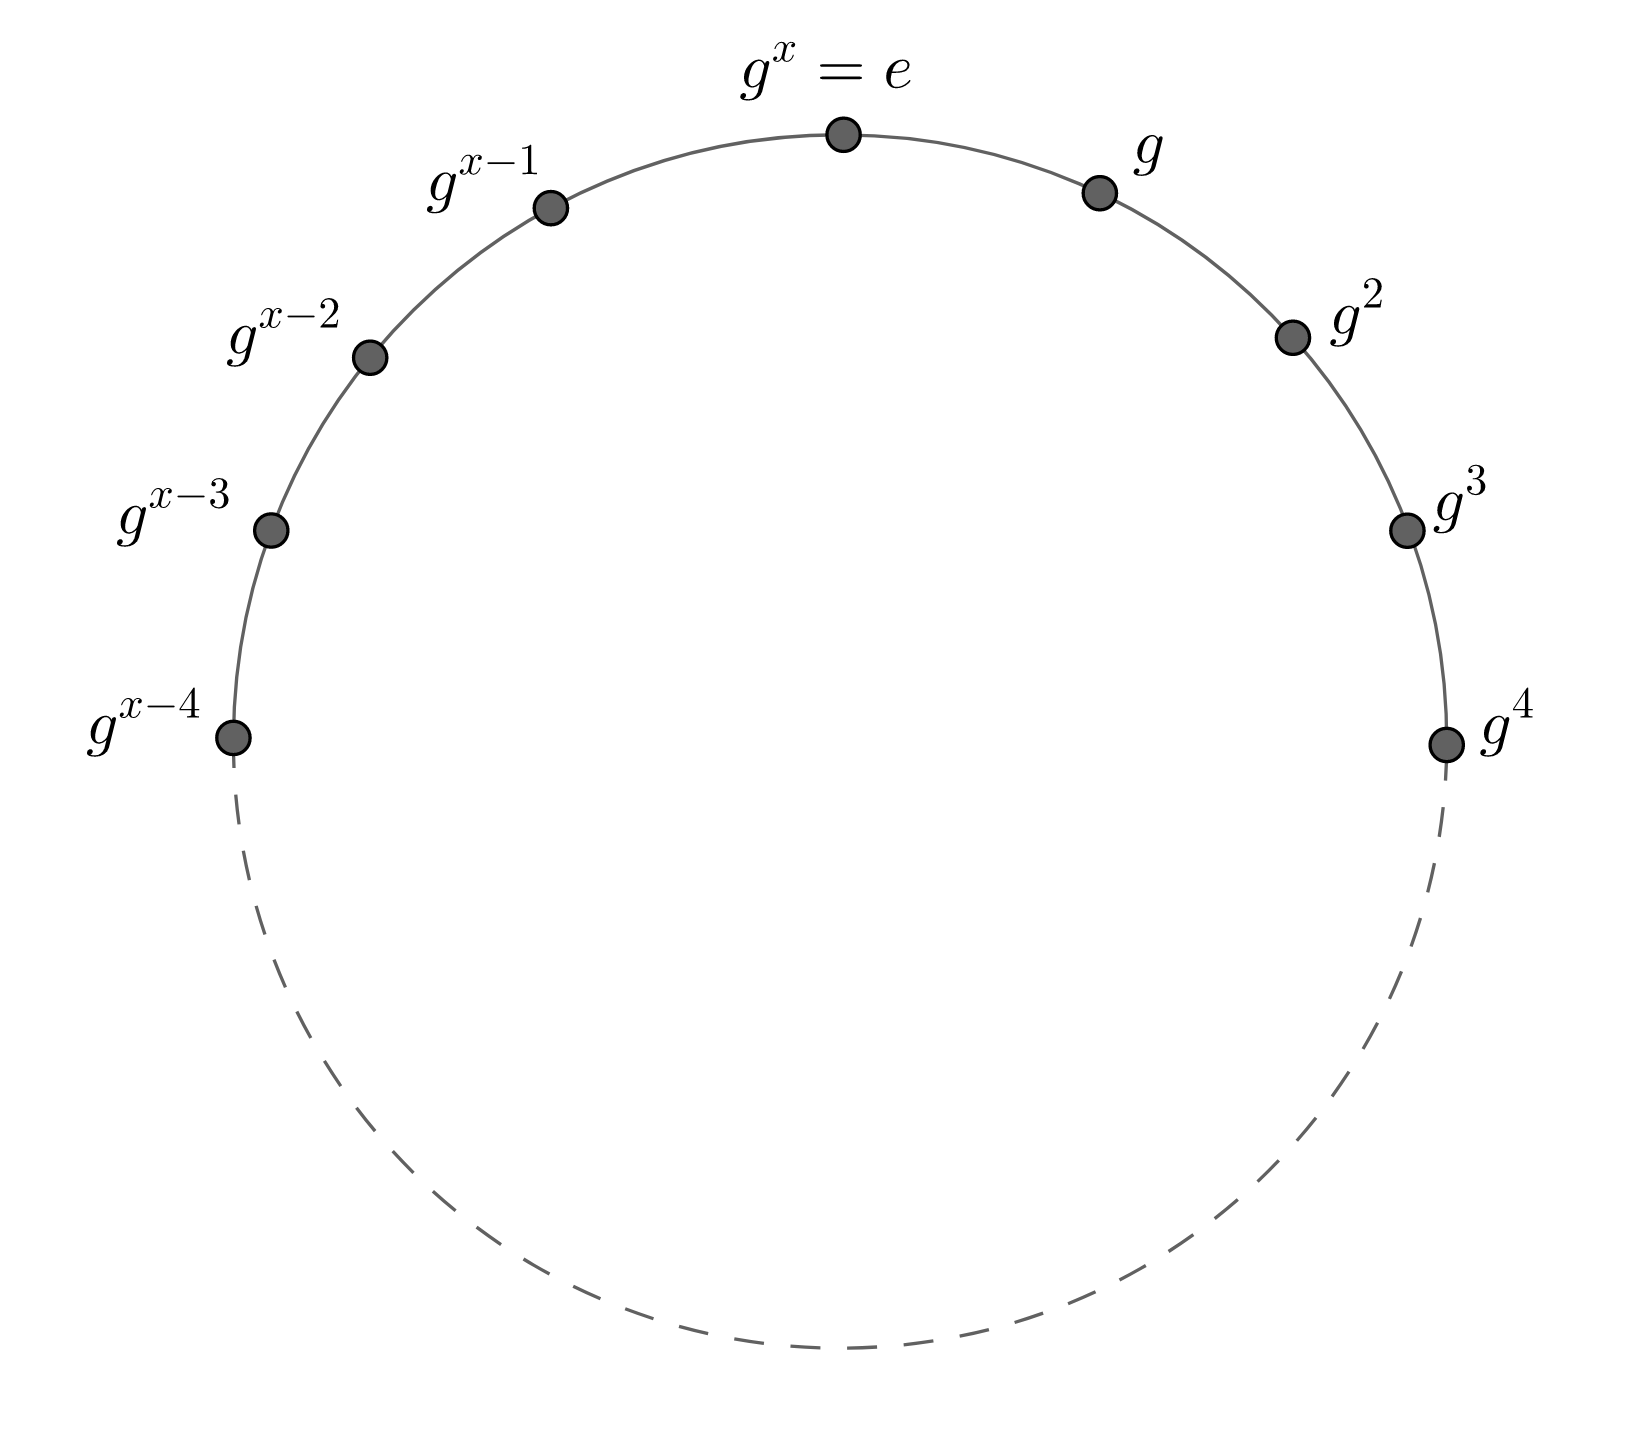
\includegraphics[width=.6\linewidth, height=.67\textheight, keepaspectratio]{Figures/cyclicgroup}
\caption{Cyclic group\index{cyclic group}\index{group}}
\label{Cyclic group}
\end{center}
\end{figure}

A a well known practice of presenting a finite group's\index{group} operation is {\em Cayley table\index{Cayley table}} as shown in example \ref{example_Cayleytable}.
Cayley table\index{Cayley table} shows all possible group operation that can be performed in a finite group.

\begin{example} \label{example_Cayleytable}
	The Cayley table\index{Cayley!Cayley table} for the group\index{group} $\mathbb{Z}_4$ is:
	\begin{center}
		\begin{tabular}{c|cccc}
			$\oplus_4$&\em 0&\em 1&\em 2&\em 3       \\
			\hline
			\em 0&\em 0&\em 1&\em 2&\em 3       \\
			\em 1&\em 1&\em 2&\em 3&\em 0       \\
			\em 2&\em 2&\em 3&\em 0&\em 1       \\
			\em 3&\em 3&\em 0&\em 1&\em 2       \\
		\end{tabular}
	\end{center}
\end{example}
In the above example of group $(\mathbb{Z}_4,+)$, there are $\phi(4)=2$ generators, $3$ and $1$.

\begin{definition}[Subgroup\index{subgroup}]
	Let $\mathbb{H}$ be  a non-empty subset  fo group $\mathbb{G}$, $\mathbb{H}$  will be called subgroup of $\mathbb{G}$ if  $\mathbb{H}$  itself follows group axioms and $\mathbb{H}$ has the same identity element of group $\mathbb{G}$. 
	\qed
\end{definition}

\begin{theorem}[Lagrange's Theorem:]
	Let $\mathbb{G}$ be a finite abelian group and $\mathbb{H}$ is a subgroup of $\mathbb{G}$.  The order of $\mathbb{G}$, $\#\mathbb{G}$ is divisible by the order of subgroup $\mathbb{H}$, $\#\mathbb{H}$ i.e.   $\#\mathbb{H} | \#\mathbb{G}$.
\qed
\end{theorem}

\begin{theorem}[Fermat’s Little Theorem:]
	Let $p$ is a prime and $a \in \mathbb{Z}$, then $$a^p = a ~(\bmod ~p)$$
	\qed
\end{theorem}
Fermat’s \textit{little theorem} is a special case of Lagrange’s theorem.


\subsection{Homomorphism in groups \index{homomorphism}}
Morphisms in groups is often used the research of cryptography and inseparable to for pairing-based cryptography research.
\begin{definition}[Homomorphism\index{rings}]
	Let $(\mathbb{G},\circ)$ and $(\mathbb{G}^{'},\star)$ be two groups with identity elements $e$ and $e'$ respectively.
	A homomorphism  is a map $f$ which preserves the group structure while the elements are mapped from $(\mathbb{G},\circ)$ to $(\mathbb{G}^{'},\star)$.
	\qed
\end{definition}
	A homomorphic map obeys the following conditions:
	\begin{itemize}
		\item $\forall a,b \in \mathbb{G}$, $f(a \circ b) = f(a) \star f(b)$.
		\item  For every $a \in \mathbb{G}$, the inverse map is $f(a^{-1}) = f(a)^{-1}$.
		\item  Identity element mapping also preserves the structure i.e. $f(e) =e'$.
	\end{itemize}

\subsubsection{Types of Homomorphism}
\begin{quote}
	\begin{description}
				\item[Isomorphism \index{Isomorphism}] If element from $\mathbb{G}$  and $\mathbb{G}^{'}$ have bijective relation then $\mathbb{G}$ and $\mathbb{G}^{'}$ are isomorphic to each other.
					
			\item[Endomorphism  \index{Endomorphism}]  If elements from group $(\mathbb{G},\circ)$ is mapped to itself then it is called endomorphism. 
			A frequently used endomorphism in cryptographic algorithms is Frobenius endomorphism. 
			
			\item[Authomorphism  \index{Authomorphism}] If element of a group has both endomorphism and isomorphism then it is called automorphism.
	\end{description}
\end{quote}

\begin{definition}[Kernel\index{kernel}]
	Let $(\mathbb{G},\circ)$ and $(\mathbb{G}^{'},\star)$ be two groups with identity elements $e$ and $e'$ respectively and $f$ is homomorphism from $(\mathbb{G},\circ)$ to $(\mathbb{G}^{'},\star)$.
	The kernel of $f$ is denoted as $\text{Ker}\{f\}$, defined by 
	$$\text{Ker}(f) = \{ a \in \mathbb{G}: f(a) = e'\}$$.
	\qed
\end{definition}

%--------------------------------------
%--------------------------------------
\subsection{Ring}
The concept of \textit{Ring} will not come as frequently as group and field in the subsequent chapters. 
However, it is relevant to define ring to understand the related concept.
\begin{definition}[Ring \index{ring}]
	A \textbf{ring} $\mathbb{R}$ is an algebraic structure with two operations, i.e. addition  $+$ and  multiplication $\cdot$  usually denote as $\mathbb{R},+,\cdot$.
	\begin{itemize}
		\item $\mathbb{R}$ is abelian group under addition operation.
		\item Under multiplication, $\mathbb{R}$ is closed and associative with identity element is $1$.
		\item  Multiplication is distributive over addition: $ \forall a, b, c \in \mathbb{R}: a\cdot (b+c) = a\cdot b + a\cdot c$.
	\end{itemize}
\qed
\end{definition}
If multiplication operation is commutative, $\mathbb{R}$  forms a commutative ring.
%\begin{example}
%	TODO
%\end{example}
\begin{definition}[Multiplicative Inverse Modulo $n$ \index{multiplicative inverse}]
	Let $\mathbb{Z}_n$ be a set under modulo $n$ and $a \in \mathbb{Z}_n$. 
	The multiplicative inverse modulo $n$ of $a$ can be written as  follows:
	$$a\cdot x \equiv  1 \bmod n.$$
The value $x$ is the multiplicative inverse modulo $n$ of $a$, often written as $a^{-1}$.
\qed
\end{definition}
Such value of $x$ only exists if $\text{gcd}(x,n)=1$.
If $n=p$ is a prime then every non-zero element in the set $\mathbb{Z}_p$ will have multiplicative inverse.
Such $(\mathbb{Z}_p,+,\cdot)$ will be a ring and having the above property it will form a field.

\subsection{Field}
\begin{definition}[Field]
	A field $(\f{},+,\cdot)$ is a set that obeys two binary operations denoted by $+$ and $\cdot$, such that:
	\begin{itemize}
%		\begin{itemize}
			\item $\f{}$ is a commutative group with respect to $+$ having identity element $0$.
			
			\item Let ${\f{\,}}^{\ast}\!\!$ is a subset of $\f{}$ having only not-zero element of $\f{}$ i.e. ${\f{}}^{\ast}  = {\f{} ~\backslash \{0\}}$. 
			Then ${\f{\,}}^{\ast}\!\!$ will be called a commutative group respect to multiplication$\cdot$  where every element should have multiplicative inverse in  ${\f{\,}}^{\ast}\!\!$.
			\item For all $a,b,c \in\f{}$  the distributive law will be followed, e.g. $a\cdot(b+c)=a\cdot b+a\cdot c$ and $(b+c)\cdot a=b\cdot a +c\cdot a$.
	\end{itemize}
%\end{itemize}
	\qed
\end{definition}
%In general, the elements $0$ and $1$ denote the unit elements regarding to addition $+$ and multiplication $\cdot$, respectively.
\begin{definition}[Subfield \index{subfield}]\hspace{0em} \label{definition_subfielf}
	Let $\f{1}$ is a subset of field $\f{}$. $\f{1}$ will be called a subfeld if $\f{1}$ itself obeys the laws of field with respect to the field operation inherited from  $\f{}$.
	\qed
\end{definition}
\begin{remark}
	 In Definition \ref{definition_subfielf}, $\f{}$ is called an {\em extension field} of $\f{1}$.
	  If $\f{1}\neq \f{}$, then $\f{1}$ is a {\em proper subfield} of $\f{}$.
 \end{remark}

\begin{definition}[Order of Finite Field \index{order of field}]\hspace{0em}
	The order is the number of elements in $\f{}$. If the order of $\f{}$ is finite, $\f{}$ is called finite field. 
	\qed
\end{definition}
\begin{definition}[Characteristic of Finite Field \index{field characteristics}]\hspace{0em}
	Let $\f{}$ be a field and smallest positive number $n$ such that $n \cdot a= 0$ for every $a\in \f{}$. Such $n$ is called characteristic. If there is no such $n$ in  $\f{}$ then $\f{}$ has characteristics $0$.
	\qed
\end{definition}

Most of the works presented in this dissertation deals with  finite fields only. 
A common property of finite fields often used in cryptographic is fllows:
\begin{theorem}\label{Cyclic Group in Finite Field}
	For every finite field $\f{}$, the multiplicative group $({\f{\,}}^{\ast}\!\!, \cdot)$ is cyclic. 
	\qed
\end{theorem}

\begin{definition}[Prime Field \index{prime field}]
	Let $p$ be a prime. The ring of integers modulo $p$ is  a finite field of characteristics $p$ having field order $p$ denoted as $\f{p}$ is called a prime field.
	 \qed
\end{definition}
\begin{remark}
		A prime field contains no proper subfield.
\end{remark}

\begin{theorem}
	Every finite field has a prime field as a subfield. \qed
\end{theorem}

In this work we classified finite fields into two types, i.e.  prime field $\f{p}$ and its extension field. 
 \secref{sec:chap:fund:extenion_field} explains more of extension field.
The prime field $\Fp$ has  the order and characteristic as $p$.
Using the modular arithmetic in the same way as Definition \ref{sec:chap:fund:extenion_field}, we can define fundamental operations of prime field $\Fp=\{0,1,2\cdots,p-1\}$.
The Cayley table will de
\begin{example}The Cayley table for the two operations $+$ and $\cdot$ for elements in $\f{5}$ are as follows:
	\begin{center}
		\begin{tabular}{c|ccccc}
			$+$&\em 0&\em 1&\em 2&\em 3&\em 4       \\
			\hline
			\em 0&\em 0&\em 1&\em 2&\em 3&\em 4       \\
			\em 1&\em 1&\em 2&\em 3&\em 4&\em 0      \\
			\em 2&\em 2&\em 3&\em 4&\em 0&\em 1      \\
			\em 3&\em 3&\em 4&\em 0&\em 1&\em 2      \\
			\em 4&\em 4&\em 0&\em 1&\em 2&\em 3      \\
		\end{tabular}\ \ 
		\begin{tabular}{c|ccccc}
			$\cdot$&\em 0&\em 1&\em 2&\em 3&\em 4       \\
			\hline
			\em 0&\em 0&\em 0&\em 0&\em 0&\em 0       \\
			\em 1&\em 0&\em 1&\em 2&\em 3&\em 4      \\
			\em 2&\em 0&\em 2&\em 4&\em 1&\em 3      \\
			\em 3&\em 0&\em 3&\em 1&\em 4&\em 2      \\
			\em 4&\em 0&\em 4&\em 3&\em 2&\em 1      \\
		\end{tabular}
	\end{center}
\end{example}
As described above, we can define arithmetic operations in $\Fp$ by modular operations ($\bmod\ p$) for integers. However, it does not work in an extension field $\F{p}{m}$. In the next section, arithmetic operations in extension field $\F{p}{m}$ is described in detail.


\section{Extension Field} 
\label{sec:chap:fund:extenion_field}
%--------------------------------------
A subset $\F{0}{}$ of a field $\F{}{}$ that is itself a field under the operations of $\F{}{}$ will be called a {\it subfield} of $\F{}{}$.
In this case, $\F{}{}$ is called an {\it extension field} of $\F{0}{}$.
An extension field of a prime field $\F{p}{}$ can be represented as $m$-dimensional vector space that has $m$ elements in $\F{p}{}$.
Let the vector space be the $m$-th extension field, it is denoted by $\F{p}{m}$.
The order of extension fields $\F{p}{m}$ is given as $p^m$. 
In what follows, let $q$ be the power of $p$, the extension field of a prime field $\F{p}{}$ is denoted by $\F{q}{}$.



There are several methods to represent an element in extension fields, such as polynomial basis and normal basis.
In this thesis, we use normal basis.
Let $\omega$ be a root of $m$-th irreducible polynomial over $\F{q}{}$, we consider the following $m$ elements.

\begin{equation}
\omega,\;\omega^q,\;\omega^{q^2},\;\cdots,\;\omega^{q^{m-1}} \nonumber
\end{equation}
All elements in this set are conjugate to each other.
When the set of the conjugates become linearly independent, this is called {\it normal basis}.
Using normal basis, an element $\alpha \in \F{q}{}$ is expressed as a polynomial by  
\begin{equation}
\alpha = a_1 \omega + a_2 \omega^q + a_3 \omega^{q^2} + \cdots + a_m \omega^{q^{m-1}}, 
\end{equation}
where $a_1,\;a_2,\;a_3,\cdots,\;a_m \in \F{q}{}$.

Arithmetic operations in $\F{q}{m}$ are carried out with ordinary addition and multiplication for polynomial and modular reduction by irreducible polynomial.

\section{Frobenius Map}
\label{sec:chap:fund:frobeniusmap}
%--------------------------------------

For any element $\alpha \in \F{q}{m}$, let us consider the following map $\pi_q:\alpha \rightarrow \alpha^q$. 
%$\F{q}{m}$‚Ì”CˆÓ‚ÌŒ³$\alpha$‚ɑ΂µ‚Ä$\pi_q:\alpha \rightarrow \alpha^q$‚Æ‚¢‚¤ŽÊ‘œ‚ðl‚¦‚éD
\begin{eqnarray}
\pi_q(\alpha) &=& \left( a_1 \omega + a_2 \omega^q + a_3 \omega^{q^2} + \cdots + a_m \omega^{q^{m-1}} \right)^q \nonumber \\ 
&=& a_1 \omega^q + a_2 \omega^{q^2} + a_3 \omega^{q^3} + \cdots + a_m \omega^{q^m} \nonumber \\
&=& a_m \omega + a_1 \omega^q + a_2 \omega^{q^2} + \cdots + a_{m-1} \omega^{q^{m-1}}
\end{eqnarray}
Note that the order of $\F{q}{m}^*$ is given by $q^m - 1$, that is,  $\omega^{q^m} = \omega$ is satisfied.
Furthermore, $a^q$ is equal to $a$ for each coefficients $a$.

Therefore, the map $\pi_q(\alpha)$ is efficiently calculated by cyclic shift operations among its basis coefficients, 
which is free from arithmetic operations.
From the computational efficiency, the map $\pi_q$ is especially called Frobenius map.

In ElGamal Encryption, many exponentiations are executed in encryption and decryption processes.
When the exponent is equal to $p$, its calculation cost can be reduced by using Frobenius map.
Therefore, Frobenius map is widely used in the cryptographic application.     

\section{Quadratic Residue/Quadratic Non-residue, \\and Cubic Residue/Cubic Non-residue}
\label{sec:chap:fund:qrqnr}
%--------------------------------------

For any non-zero element $d\in\F{q}{}$, $d$ is called a Quadratic Residue (QR) when $x$ such that $x^2=d$ exists in $\F{q}{}$.
On the other hand, when such an $x$ does not exist in $\F{q}{}$, $d$ is called a Quadratic Non-Residue (QNR).
We can identify whether or not $d$ is a QR by following test.

\begin{eqnarray}
d^{(q-1)/2} = \left\{
\begin{array}{ll}
1 & \mbox{: QR} \\
-1 & \mbox{: QNR} 
\end{array}
\right.
\end{eqnarray}

All elements in finite fields $\F{q}{}$ of odd characteristics become QR in extension fields $\F{q}{2j}$.
On the other hand, quadratic non-residues also become QNR in $\F{q}{i}$, where $i$ is not divisible by 2.


\section{Elliptic Curve}
\label{sec:chap:fund:ecc}
In this section, we review elliptic curves and pairings. 

%--------------------------------------
\subsection{Additive Group over Elliptic Curves}
%--------------------------------------

In general, let $p>3$, an elliptic curve $E/\F{p}{}$ over a finite field $\F{p}{}$ is defined as 

\begin{equation}
E/\F{p}{}: y^2=x^3+ax+b,\ 42a^3+27b^2 \neq 0,\ a,b\in \F{p}{}. \label{EC}
\end{equation}

The field that $x$ and $y$ belong to is called the definition field. 
The solutions $(x,y)$ of \eqref{EC} is called rational points.
$E(\F{q}{})$ that is the set of rational points on the curve, including the {\it point at infinity} $\mathcal{O}$, forms an additive abelian group. 
The {\it point at infinity} works as an unity element in $E(\F{q}{})$.
When the definition field is $\F{q}{m}$, we denote the additive group by $E(\F{q}{m})$.

For rational points $P_1(x_1,y_1)$, $P_2(x_2,y_2)$ $\in E(\F{q}{})$, the elliptic curve addition $P_3(x_3,y_3)=P_1+P_2$ is defined as follows.
\begin{eqnarray*}
	\lambda &=& \left\{ \begin{array}{ll}
		{\displaystyle \frac{y_2-y_1}{x_2-x_1}} & P_1\neq P_2,\ x_1\neq x_2 \\
		& \\
		{\displaystyle \frac{3x_1^2+a}{2y_1}} & P_1=P_2 \\
		
	\end{array} \right.\\
	x_3 &=& \lambda^3-x_1-x_2\\
	y_3 &=& (x_1-x_3)\lambda-y_1
\end{eqnarray*} 
%In the case of $P_1=P_2$, the addition is especially called elliptic curve doubling. 
$\lambda$ is the tangent at the point on the curve and $\cal O$ is the additive unity in $E(\f{p})$.
In what follows, If $P_1 \neq P_2$ then $P_1+P_2$ is called elliptic curve addition (ECA). 
If $P_1=P_2$ then $P_1+P_2=2P_1$, which is known as elliptic curve doubling (ECD). 
%Let $\#E(\F{p}{})$ be its order, consider a large prime $r$ that divides $\#E(\F{p}{})$. %The smallest positive integer $k$ such that $r$ divides $p^k-1$ is called {\it embedding degree}. One can consider pairings such as Tate and Ate pairings by using $E(\F{p}{k})$. 

Let a rational point $P(x,y)$, an inverse point $-P$ is given by $-P(x, -y)$. 
Elliptic curve cryptographies is constructed on elliptic curve groups $E(\F{q}{})$.



Let $\#E(\F{p}{})$ be the order of $E(\F{p}{})$, it is given as
\begin{equation}
\#E(\F{p}{})=p+1-t, %abel{order}
\end{equation}
where $t$ is the Frobenius trace of $E(\F{p}{})$. 

From Hasse's theorem, $t$ satisfies
\begin{equation}
|t| \leq 2\sqrt{p}.
\end{equation}

\subsection{Scalar Multiplication in Elliptic Curve}
\label{sec:chap:fund:scm}
Let $[s]P$ denote the $(s-1)$-times addition of a rational point $P$ as, 
\begin{equation}
[s]P = \sum_{i = 0}^{s-1}{P}.
\end{equation}
This operation is called a scalar multiplication.
As a general approach for accelerating a scalar multiplication, the binary method is the most widely used.

\paragraph{Binary method}
\label{sec:chap:fund:binscm}
The binary method is an extensively applied method for calculating the elliptic curve scalar multiplication. 
 The pseudo code of left-to-right binary scalar multiplication algorithm is shown in \algref{alg:binary_scm_chap_fundamental}. 
 This algorithm scans the bits of scalar $s$ from the  most significant bit to the least significant bit. When $s[i] = 1$, it  performs ECA and ECD otherwise only ECD is calculated. 
 The binary method iterates elliptic curve doublings and elliptic curve additions using binary representation of scalar.
 A scalar multiplication needs $\lfloor \log_2 s\rfloor$ elliptic curve doublings and $\lfloor \log_2 s\rfloor/2$ elliptic curve additions on average.
  This method is easy to implement but the important drawback of this method is not resistant to \textit{side channel attack} \cite{C:Kocher96}.  

\begin{algorithm}[ht]
	\caption{Left-to-right binary algorithm for elliptic curve scalar multiplication}
	\label{alg:binary_scm_chap_fundamental}
	\DontPrintSemicolon
%	\hspace{-3ex}
	\KwIn{ $P$, $s$}
%	\hspace{-3ex}
	\KwOut{$[s]P$} %output
	 $T$ $ \leftarrow$ $0$ \;
	 \For{$i = \lfloor \log_2 s \rfloor$ {\bf to} $0$} {\;
				$T \leftarrow T  + T$\;
		    \If{ $s[i] = 1$}{
			      $ T \leftarrow T + P$\;
	} }
	 \text{return} $T$\;
\end{algorithm}

\paragraph{Montgomery ladder method}
\label{sec:chap:fund:montscm}
Montgomery ladder algorithm is said to be resistant to \textit{side channel attack}. Such resistance comes by paying tolls as calculation overhead which slows down this method than binary method.  \algref{alg:mont_scm_chap_fundamental} shows the Montgomery ladder algorithm for scalar multiplication. Montgomery ladder has some similarity with binary method except in each iteration it performs ECA and ECD. 

\begin{algorithm}[ht]
	\caption{Montgomery ladder algorithm for elliptic curve scalar multiplication}
	\label{alg:mont_scm_chap_fundamental}
	\DontPrintSemicolon
%	\hspace{-3ex}
	\KwIn{ A point $P$,  an integer $s $}
%	\hspace{-3ex}
	\KwOut{$[s]P$} %output
	 $T_0$ $ \leftarrow$ $0$, $T_1$ $\leftarrow$ $P$ \;
	 \For{$i = \lfloor \log_2 s \rfloor$ {\bf to} $0$} {\;
		  \If{ $s[i] =1$}{
			         $ T_0 \leftarrow T_0 + T_1$\;
			     $T_1 \leftarrow T_1 + T_1$\;
		}
		        {\ElseIf{$s[i] = 0$}{ 
				      $T_1 \leftarrow T_0 + T_1$\;
				  		 $T_0 \leftarrow T_0 + T_0$\;}
		}
	}
	 \text{return} $T_0$\;
\end{algorithm}

\paragraph{Sliding-window Method}
\label{sec:chap:fund:swscm}
Sliding-window \cite{DBLP:reference/crc/2005ehcc} algorithm is also resistant to \textit{side channel attack} and at the same  time it is faster than Montgomery ladder. In this method the scalar $s$ is processed in blocks of length $w$, known as window size. \algref{alg:sw_scm_chap_fundamental} shows the sliding-window algorithm for scalar multiplication.

\begin{algorithm}[ht]
	\caption{Sliding window algorithm for elliptic curve scalar multiplication}
	\label{alg:sw_scm_chap_fundamental}
	\DontPrintSemicolon
%	\hspace{-3ex}
	\KwIn{ A point $P$,  an integer $s = \sum_{j=0}^{l-1} s_j2^{j} $, $s_j \in \left\lbrace 0,1 \right\rbrace$, window size $w \geq 1$} 
%	\hspace{-3ex}
	\KwOut{Q = $[s]P$} 
	\textit{Pre-computation.} \; 
	 $P_1\leftarrow P$, $P_2 \leftarrow [2]P$ \;
	 \For{$i = 1$ {\bf to} $2^{w-1}-1$} { $P_{2i+1} \leftarrow P_{2i-1} + P_2$}\;
	 $j \leftarrow l-1$, $Q \leftarrow \cal{O}.$\;
	\textit{Main loop.}\;
	 \While{$j \geq 0$} {\;
		 \If{ $s_j =0$}{
			$Q \leftarrow [2]Q$, $j \leftarrow j-1$\;
		}
		            \Else{\;
			 Let $t$ be the least ineger such that \;
			$j - t+1 \leq w$ and $s_t =1$\;
			 $h_j \leftarrow (s_js_{j-1} \cdots s_t)_2$\;
			 $Q \leftarrow [2^{j-t+1}]Q +P_{h_j}$      \;      
			 $j \leftarrow t-1$ \;
		}
	}
	 return $Q$
\end{algorithm}

%--------------------------------------
\subsection{Frobenius Map on Elliptic Curve Groups}
%--------------------------------------
In this section, we introduce Frobenius map for a rational point in $E(\F{q}{})$.
For any rational point $P=(x, y)$, Frobenius map $\phi$ is given by $\phi:P(x, y) \rightarrow ({x}^q, {y}^q)$.
Then, the following relation holds for any rational points in $E(\F{q}{})$ with regard to Frobenius map.
\begin{equation*}
\left(\phi^{2}-[t]\phi+[q]\right)P=\mathcal{O}.
\end{equation*}
Thus, we have
\begin{equation}
[q]P=\left([t]\phi-\phi^2\right)P. \label{frobscm}
\end{equation}
From Hasse's theorem, note the bit-size of Frobenius trace $t$ is about a half of the characteristic $p$. 
Using \eqref{frobscm}, we can efficiently calculate scalar multiplication \cite{C:Koblitz91}.

\section{Definition of Pairing} \label{secDefPairing} %\label{tp}

%--------------------------------------
\subsection{Properties of Pairing}
%--------------------------------------
%--------------------------------------
\subsection{Pairing-friendly Curves}\label{sec:pfc}

\subsubsection{Barreto-Neahrig Curve}

\subsubsection{Barreto-Neahrig Curve}



%--------------------------------------
\subsection{Tate Pairing}
%--------------------------------------

%--------------------------------------
\subsection{Ate Pairing}

\subsection{Optimal-Ate Pairing}



%--------------------------------------
\subsection{Miller's Algorithm}
%--------------------------------------

	%--------------------------------------
	\subsection{Final Exponentiation}
	%--------------------------------------
	
	
	
	\section{Conclusion}
	This chapter briefly reviewed the mathematical fact to define the pairing, and shows a target class of elliptic curves.
	In addition, we described the conventional pairings such as Tate, Ate, and {\it twisted} Ate pairings.
	
	

